\documentclass[crop,tikz,border=1px]{standalone}
\renewcommand{\familydefault}{\sfdefault}

\usetikzlibrary{calc,arrows,positioning,scopes,shapes,matrix}

\begin{document}
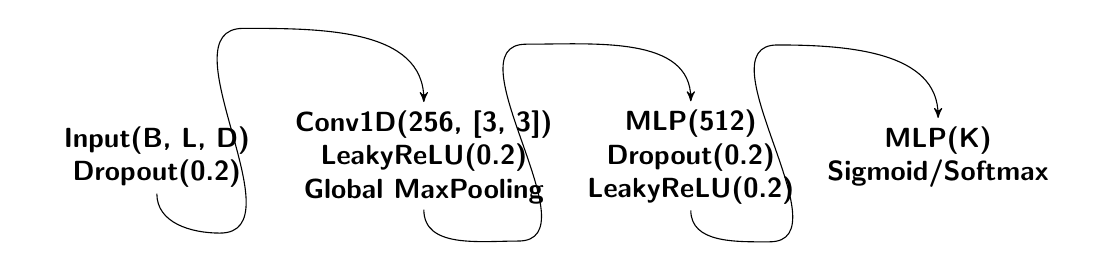
\begin{tikzpicture}[->,>=stealth',shorten >=1pt,auto,node distance=2.5cm,inner
 sep=2pt, every node/.style={rectangle,text width=3cm,anchor=center,align=center,font=\bf}]

  \matrix[matrix of nodes] (m) {
    {Input(B, L, D)\\Dropout(0.2)} &
    |[text width=3.5cm]|{Conv1D(256, [3, 3])\\LeakyReLU(0.2)\\Global MaxPooling} &
    {MLP(512)\\Dropout(0.2)\\LeakyReLU(0.2)} &
    {MLP(K)\\Sigmoid/Softmax} \\
  };

  \path[draw] (m-1-1.south) to[out=-90,in=180] +(0.8,-0.5) to[out=0,in=180]
  +(1.1,2.1) to[out=0,in=90] (m-1-2.north);

  \path[draw] (m-1-2.south) to[out=-90,in=180] +(1.2,-0.4) to[out=0,in=180]
  +(1.3,2.1) to[out=0,in=90] (m-1-3.north);

  \path[draw] (m-1-3.south) to[out=-90,in=180] +(1.0,-0.4) to[out=0,in=180]
  +(1.1,2.1) to[out=0,in=90] (m-1-4.north);

\end{tikzpicture}
\end{document}